\begin{figure}[h]
\centering
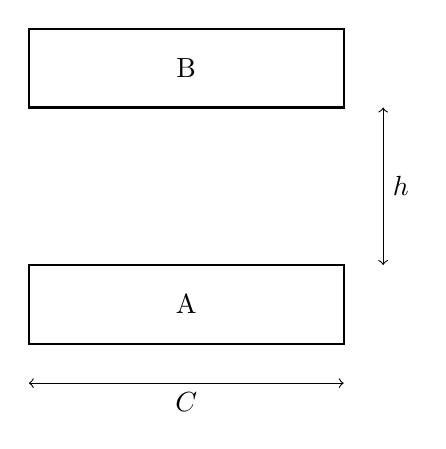
\begin{tikzpicture}[scale=1]

    % Shape B (top)
    \draw[thick] (0,0) rectangle (4,1);
    \node at (2,0.5) {B};

    % Shape A (bottom)
    \draw[thick] (0,-3) rectangle (4,-2);
    \node at (2,-2.5) {A};

    % Vertical distance h
    \draw[<->] (4.5,-2) -- (4.5,0) node[midway, right] {$h$};

    % Horizontal distance C
    \draw[<->] (0,-3.5) -- (4,-3.5) node[midway, below] {$C$};

\end{tikzpicture}
\end{figure}